\begin{multicols*}{2}

\tikz[remember picture,overlay] \node[opacity=1,inner sep=0pt] at (page cs:-0.5,-0.35){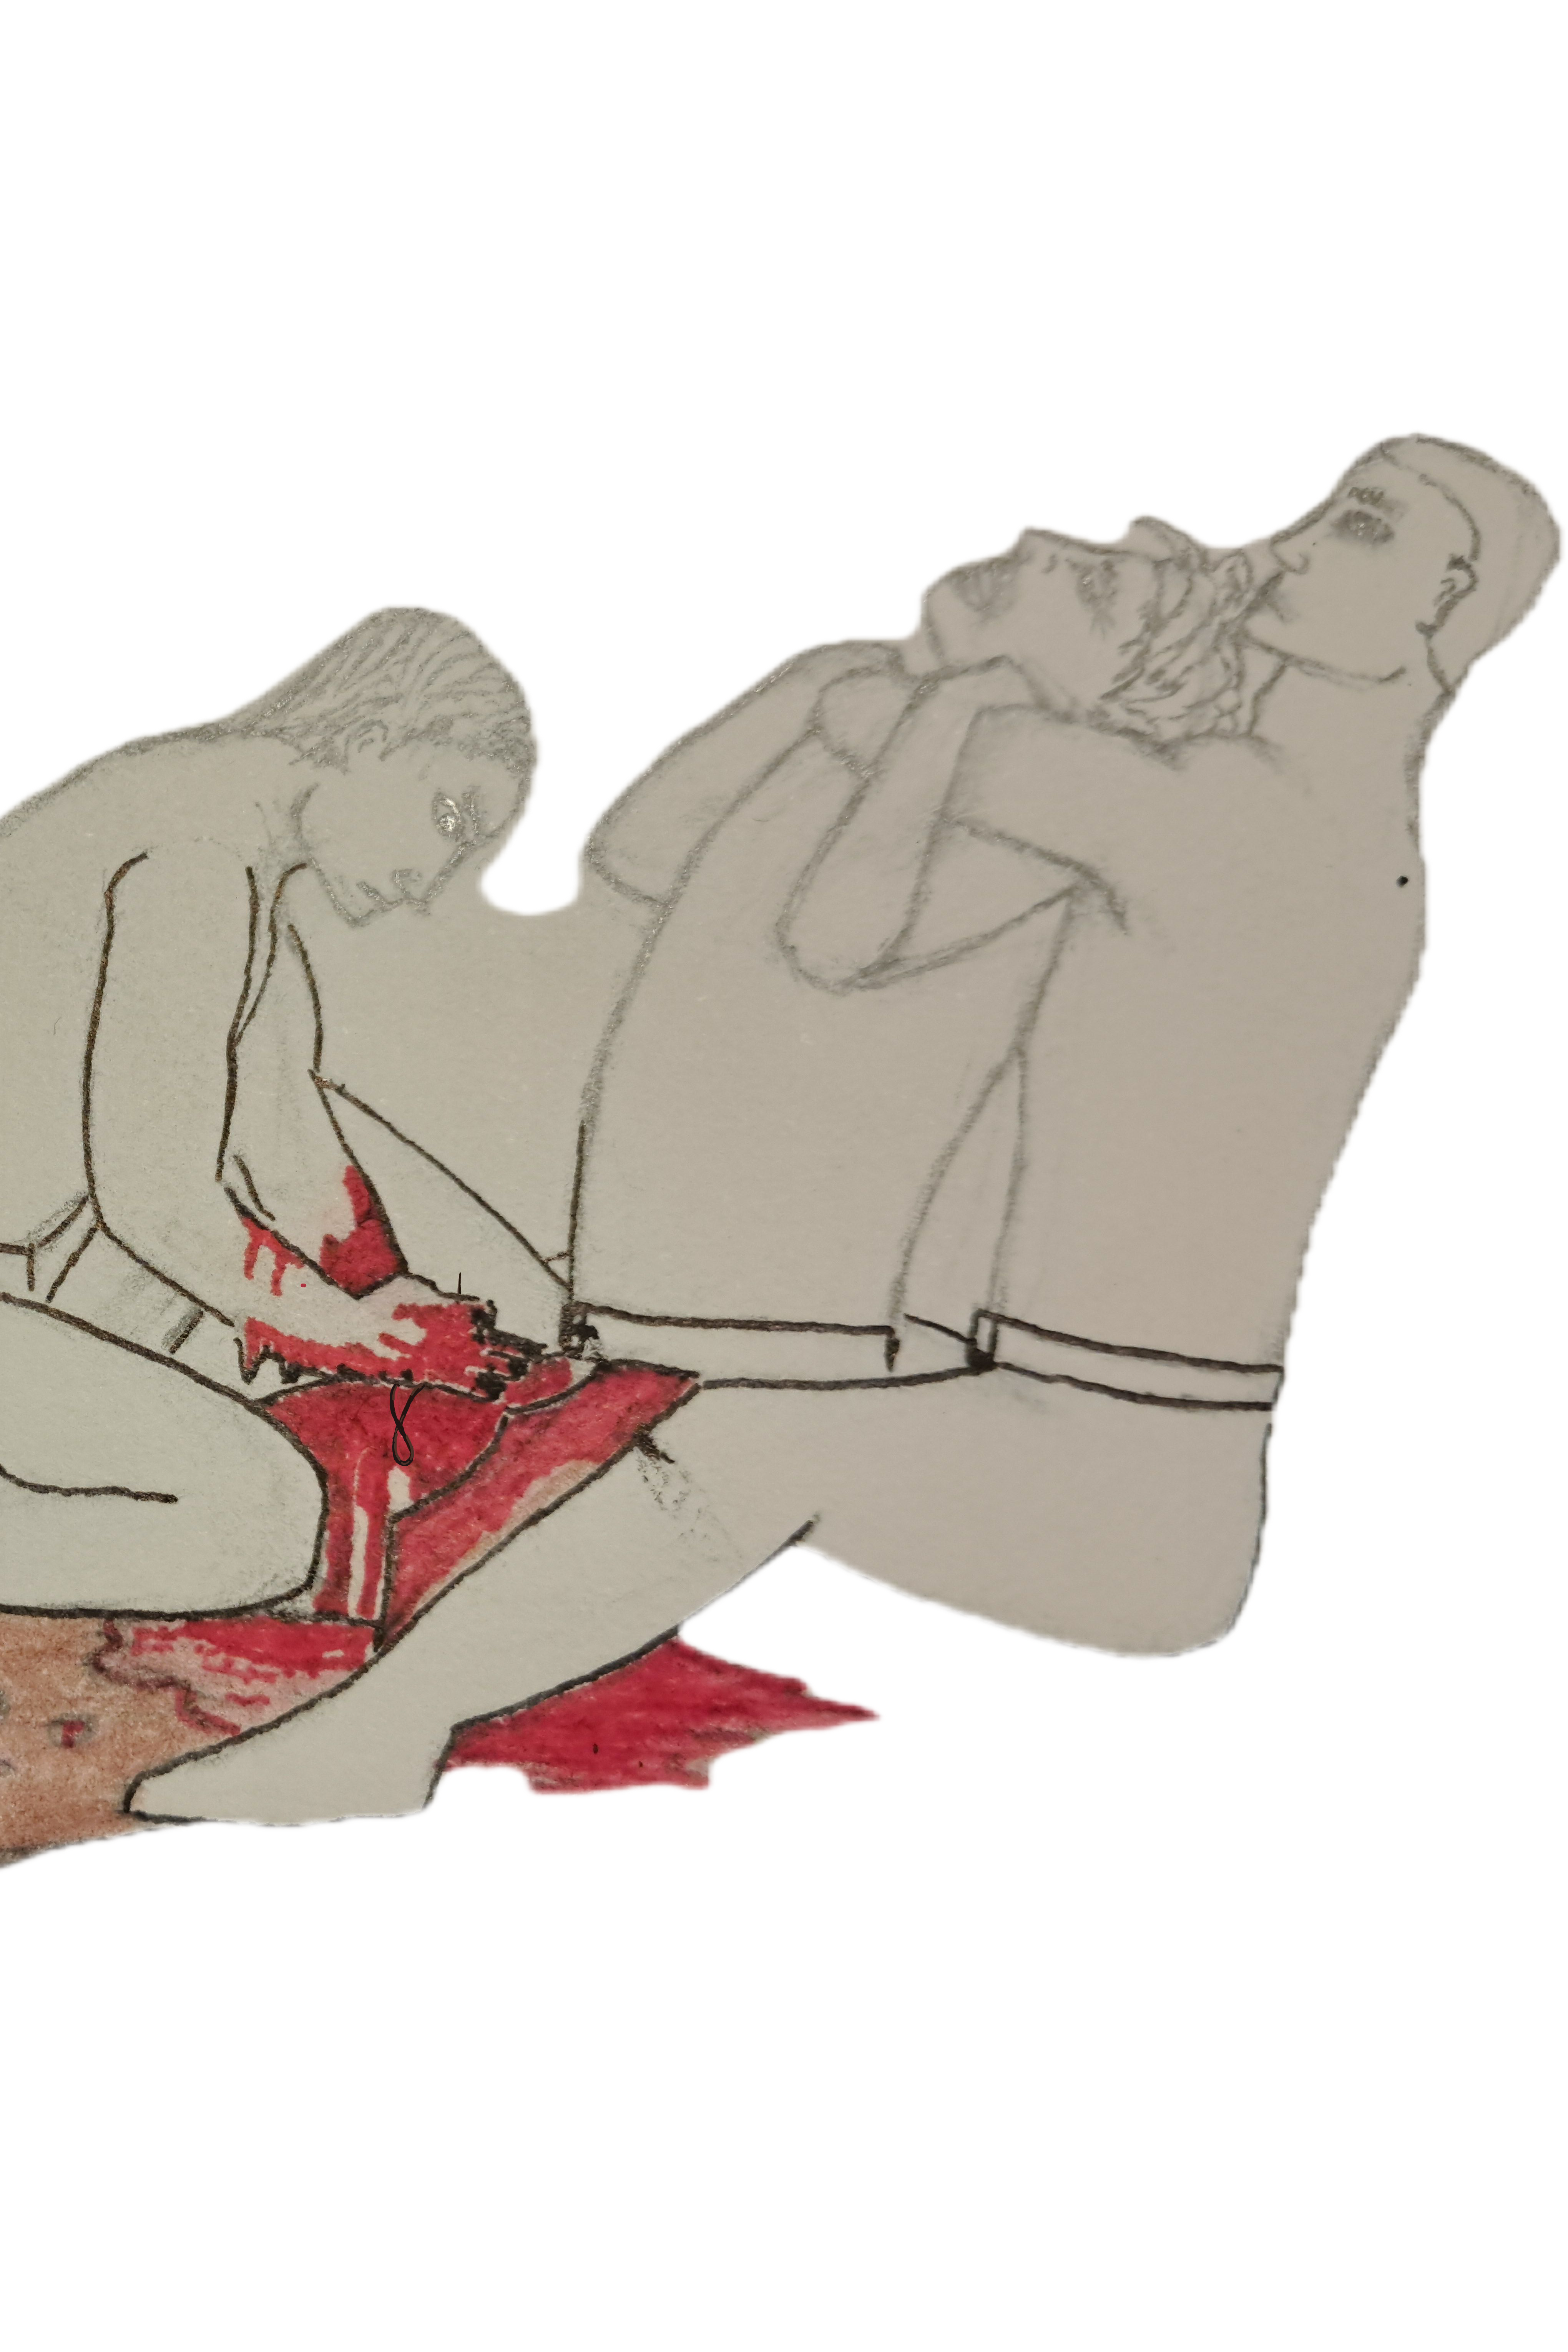
\includegraphics[width=0.5\paperwidth]{media/healing-cropped-1.png}};

\subsection*{Afflication}

For \texttt{Severe Injury} see the table below. 

\begin{center}
  \rowcolors{2}{gray!25}{white}
    \label{sec:affliction}
    \begin{tabular}{|c|p{6.4cm}|}
        \hline
        \textbf{Roll d4} & \textbf{Affliction} \\
        \hline
        \texttt{1} & The cut is deep, you are \texttt{Bleeding}:\newline lose \texttt{1} \texttt{Vigor} when your turn starts\\
        \texttt{2} & Pain is unbearable, you are in \texttt{Agony}:\newline lose \texttt{1} \texttt{Clarity} when your turn starts\\
        \texttt{3} & Grievous wound, you are in \texttt{Distress}:\newline lose \texttt{1} \texttt{Spirit} when your turn starts\\
        \texttt{4} & Luck is on your side: no Affliction.\\
        \hline
    \end{tabular}
\end{center}

For \texttt{Lethal Injuries} you lose \texttt{1d4} of corresponding virtue instead of \texttt{1}.

\subsection*{Trauma} 
When \texttt{Stress} reaches the limit a knight can sustain, it causes \texttt{Trauma}: a footprint of a great effort in the form of a mental wound.
\texttt{Trauma} fills an \texttt{Injury slot} and kills the knight by a heart attack if they are out of them.
It has neither damage die nor \texttt{Afflication} and is not considered an \texttt{Injury}.

\newcolumn

\subsection*{Healing}
\label{sec:healing}

\paragraph{Healing an Injury} removes it completely.
This is a tricky endeavour which usually requires a professional to accomplish and comes with a price tag.

Still, in dire circumstances, a knight can attempt to heal themselves or another knight:

\colbox{
\begin{enumerate}[nosep, leftmargin=*]
    \item The \textbf{healing} knight rolls a \texttt{Clarity} save to determine how to treat this type of \texttt{Injury} most effectively.
    \item The \textbf{healed} knight rolls a \texttt{Spirit} save to see if the are able to withstand the pain.
\end{enumerate}
}
Only if both of the above saves are successful, the knight is healed from the \texttt{Injury}.
Any one knight can endure only \texttt{1} healing attempt per day.

\paragraph{Getting tougher and acquiring quirks.} After suffering through the agony of medicine without painkillers, a knight is relieved from an injury completely.

If the maximum \texttt{Guard} of a knight is less than the maximum value on a die that is marked on the \texttt{Injury Slot}, increase \texttt{Guard} by \textbf{1}.

Free the \texttt{Injury Slot} that was occupied by the healed \texttt{Injury}.

Choose or make the Referee choose a \texttt{Quirk} (p.\pageref*{sec:quirks}) for you and permanently add it to your knight.

\paragraph{Dealing with Trauma} removes it completely. 
During your sleep, pass a \texttt{Clarity} and a \texttt{Spirit} save to successfully deal with \texttt{Trauma}. 
For each \texttt{Trauma} you have, treat those \texttt{Virtue} saves as if they were opposed with an additional \texttt{Focus}.

Trauma leaves a permanent mark: acquire a \texttt{Quirk}(p.\pageref*{sec:quirks}) as if a knight healed from an \texttt{Injury}.



\end{multicols*}
